% \include{header_p2.tex}

\documentclass[pre,aps,floatfix,10pt,superscriptaddress, notitlepage]{revtex4-1}
\pdfoutput=1
\usepackage[english]{babel}
\usepackage[T1]{fontenc}
\usepackage[latin9]{inputenc}
\usepackage{amsmath,amssymb}
\usepackage[svgnames]{xcolor}
\usepackage{graphicx}
\usepackage{acro}
\usepackage{subfig}
\usepackage{caption}
\graphicspath{{../figures/}}

\captionsetup[figure]{justification=raggedright}

\newcommand{\set}[1]{\ensuremath{\mathcal{#1}}}

\DeclareAcronym{pdf}{
  short=PDF,
  long=Probability Density Function,
}
\DeclareAcronym{iid}{
  short=i.i.d.,
  long=Independent Identically Distributed
}
\DeclareAcronym{ou}{
  short=OU,
  long=Ornstein-Uhlenbeck,
}
\DeclareAcronym{gktl}{
  short=GKTL,
  long=Giardina-Kurchan-Tailleur-Lecomte,
}
\DeclareAcronym{ams}{
  short=AMS,
  long=Adaptive Multilevel Splitting,
}
\DeclareAcronym{tams}{
  short=TAMS,
  long=Trajectory Adaptive Multilevel Splitting,
}
\DeclareAcronym{scgf}{
  short=SCGF,
  long=Scaled Cumulant Generating Function,
}
\DeclareAcronym{lbm}{
  short=LBM,
  long=Lattice Boltzmann Method,
}
\DeclareAcronym{lbe}{
  short=LBE,
  long=Lattice Boltzmann Equation,
}
\DeclareAcronym{lgca}{
  short=LGCA,
  long=Lattice Gas Cellular Automata,
}
\DeclareAcronym{lbgk}{
  short=LBGK,
  long=Lattice Bhatnagar-Gross-Krook
}
\DeclareAcronym{OU}{
  short=OU,
  long=Ornstein--Ulhenbeck
}
\DeclareAcronym{dns}{
  short=DNS,
  long=Direct Numerical Simulation,
}
\DeclareAcronym{md}{
  short=MD,
  long=Molecular Dynamics,
}
\DeclareAcronym{cfd}{
  short=CFD,
  long=Computational Fluid Dynamics,
}

\begin{document}
\title{A statistical mechanics approach to the simulation of extreme fluctuations of the time-averaged drag acting on an obstacle immersed in a turbulent flow}

\author{Thibault Lestang}
\email{thibault.lestang@ens-lyon.fr}
\affiliation{Univ Lyon, ENS de Lyon, Univ Claude Bernard, CNRS, Laboratoire de Physique, F-69342 Lyon, France}
\affiliation{Univ Lyon, Ecole Centrale de Lyon, Univ Claude Bernard, CNRS, Laboratoire de M\'ecanique des Fluides et d'Acoustique, F-69134 Ecully cedex, France}
\author{Freddy Bouchet}
\email{freddy.bouchet@ens-lyon.fr}
\affiliation{Univ Lyon, ENS de Lyon, Univ Claude Bernard, CNRS, Laboratoire de Physique, F-69342 Lyon, France}
\author{Emmanuel L�v�que}
\email{emmanuel.leveque@ec-lyon.fr}
\affiliation{Univ Lyon, Ecole Centrale de Lyon, Univ Claude Bernard, CNRS, Laboratoire de M\'ecanique des Fluides et d'Acoustique, F-69134 Ecully cedex, France}
\maketitle
\section{Introduction}

\section{Description of the test case for extreme drag fluctuations sampling}
\label{sec:test_flow}

\begin{figure}
  \centering
  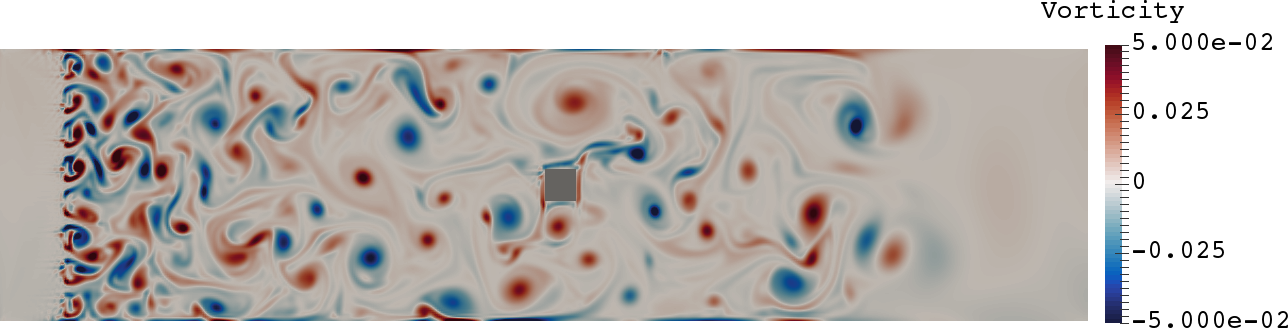
\includegraphics[width=\linewidth]{illustration_vorticity_tf2}
  \caption{Typical vorticity field in the computational domain. The square obstacle is represented by the gray area in the center of the channel.}
\end{figure}
%% Description de la g�om�trie
We consider the interaction of a two dimensional turbulent channel flow with a square cylinder, illustrated in figure~\ref{fig:computational_domain}.
At the inlet of the channel, a constant parabolic velocity profile is imposed.
We note $u_0$ the imposed fluid velocity at the inlet, at the center of the channel.
Shortly after the inlet, the flow interacts with a grid, thus leading to turbulence.
Generated eddies are advected downstream by the mean-flow and grow in size along the way---a consequence of the inverse energy cascade taking place in two-dimensional turbulent flows.
A square obstacle is mounted in the channel.
Its distance from the grid is such that the typical size of the eddies it interacts with is close to the siye of the obstacle itself.
Fluid structures are then advected further downstream where they are damped in a region of increasing viscosity, a so-called \textit{sponge layer}~\cite{ref1,ref2}.
The outlet is modelled as an open boundary, where a zero momentum flux along the mean-flow direction in imposed.

%% M�thode Boltzmann sur r�seau
The flow dynamics are computed by means of the \ac{lbm}~\cite{ref1,ref2}.
[[Paragraphe LBM]]

\subsection{The drag force}
\label{sec:drag_force}

%% Descritpion d'une fluctuations de train�e typique
The interaction of the incoming turbulent flow with the square obstacle results in fluctuating mechanical efforts exterted on the obstacle.
In particular, the \textit{drag force} is defined as the result of both pressure and viscous efforts, projected along the mean-flow direction, that is
\begin{equation}
  \label{eq:drag_definition}
  f_d = \int_{\mathcal{S}}(-p(\boldsymbol{x})\boldsymbol{I} + \boldsymbol{\tau}) \mathrm{d}\boldsymbol{\mathcal{S}} \cdot \boldsymbol{e}_x
\end{equation}
where $\mathcal{S}$ is the surface of the obstacle, $p(\boldsymbol{x})$ is the pressure acting at location $\boldsymbol{x}$, $\boldsymbol{I}$ the identiy matrix, $\boldsymbol{\tau}$ the viscous stress tensor and $\boldsymbol{e}_x$ is the unit vector pointing in the mean-flow direction.
to the formation of boundary layers at the top and bottom boundaries of the obstacle.
Figure~\ref{fig:typical_drag_signal} illustrates the time evoluction of the drag acting on the square obstacle.
\begin{figure}
  \centering
  \includegraphics[width=0.7\linewidth]{illustration_signal_drag_1}
  \caption{Typical temporal evolution of the drag acting on the square cylinder pictured in figure~\ref{fig:computational_domain}. The correlation time $\tau_c$ is defined further in this text and correspond to the typical fluctuation timescale of the drag.}
  \label{fig:typical_drag_signal}
\end{figure}
The value of the drag $f_d$ mainly depends on the local pressure and velocity gradients fields in the vicinity of the obstacle.
Furthermore, we observed that the contribution of viscous stresses to the overall drag is three order of magnitudes smaller than the contrbution of pressure.
This a consequence of the blunt shape of the ostacle, that results in an important pressure difference between the forebody (the upstream boundary) and the base (the downstream boundary).
As a result, the drag acting on the square cylinder is very well approximated by
\begin{equation}
  \label{eq:drag_approx}
  f_d(t) = p_{fb}(t) - p_{base}(t)
\end{equation}
where $p_{fb}(t)$ amd $p_{base}(t)$ denote the pressure integrated over the forebody and the base, respectively.

The typical timescale of variation of the drag is therefore corresponds to the typical timescale of variation of the pressure in the vicinity of the obstale.
It can be estimated by the \textit{turnover time}
\begin{equation}
  \label{eq:turnover_time}
  \tau_0 = \frac{R}{U}
\end{equation}
where $R$ is the diamenter of the cylinder and $U$ the mean-flow velocity.

%% The phenomenology of typical drag fluctuations

Figure~\ref{fig:typical_drag_fluctuation} illustrate the evolution of the vorticity field in the vicinity of the obstacle.
Over a few turnover times, boundary layers form along the top and bottom boundaries.
The generated vorticity turns into eddies that are advected downstream by the mean flow.
As the result, the vorticity generated along the top and bottom boundary layers have a very small impact
on the the pressure field in the vicinity of the base of the obstacle.
As result, typical fluctuations of the drag are mostly due to the fluctating pressure in the vicinity of the upstream side of the obstacle.
Such fluctuating pressure directly orginates from the incoming turbulent flow.
In the following section~\ref{sec:direct_sampling}, we illustrate very different dynamics for \textit{extreme} fluctuations of the drag acting on the obstacle.
In particular, we show that extreme fluctuations primarily result from fluctuations of the base pressure, whereas forebody pressure fluctuations play very little role.

\subsection{The drag random process: Probability Density Function, time correlations}
\label{sec:pdfs}

\begin{figure}
  \centering
    \subfloat[\ac{pdf} for the drag fluctuations $f'_d$]{\label{fig:pdf_drag_a}\includegraphics[width=.5\linewidth]{../figures/pdf_drag_SQ_asymetry_expo}}
    \subfloat[Autocorrelation function of the the instantaneous drag $f_d$]{\label{fig:pdf_drag_b}\includegraphics[width=.5\linewidth]{../figures/correlation_with_log}}  
  \caption{\textbf{(a)} \ac{pdf} describing the statistics of the instantaneous drag fluctuations $f'_d = (f_d - \bar{f_d})/\sigma$. This \ac{pdf} has been estimated on the basis of a timeseries spanning $T_{tot} = 10^6 \tau_c$. $\bar{f_d}$ and $\sigma$ denote the average and the standard deviation computed over the whole timeseries, respectively. The linear fits highlight the exponential behaviour of the the \ac{pdf} for rare events. \textbf{(b)} Autocorrelation function for the instantaneous drag $f_d$, defined as $(\mathbb{E}[f_d(t+\tau)f_d(t)]-\mathbb{E}[f_d]^2)/\sigma^2$ and estimated from a timeseries spanning $T_{tot} = 10^6 \tau_c$. This figure shows the exponential decay of the correlations over time.}
  \label{fig:pdf_drag}
\end{figure}

In the following we consider the drag force acting on the obstacle as a scalar random process $f_d(t)$.
Figure~\ref{fig:pdf_drag} displays an estimate of the \ac{pdf} for the drag process, computed on the basis of a very long timeseries $\{f_d(t)\}_{0\leq t \leq T_{tot}}$ with $T_{tot} \approx 4\times 10^{6}\tau_0$.
Two comments are in order:
\begin{itemize}
\item The probabilty is skewed towards positive fluctuations. As an indication, the skewness coefficient is ??.
\item The tails of the distribution are well described by an exponential \ac{pdf}, \textit{i.e.} $\mathbb{P}(f_d=f) \propto e^{-\alpha f}\mathrm{d}f$.
\end{itemize}
The interaction of the flow is responsible for this particular shape of the \ac{pdf}.
This can be seen by considering the flow \textit{without} obstacle, and computing the \ac{pdf} of the drag acting on a control surface corresponding to the surface of the obstacle.
This experiment is depicted in figure~\ref{fig:no_square}.
One can see in figure~\ref{fig:pdf_drag} that the \ac{pdf} of the drag process exhibits a very different shape when no obstacle interacts with the flow.
In particular, it is symmetric and does not display exponential tails.
The exponential behaviour of the \ac{pdf} describing rare events plays an important role in the description of the phenomenology of extreme fluctuations of the \textit{time-averaged} drag.
This topic is further discussed in section~\ref{sec:avg_drag}.

Figure~\ref{fig:correlation_function} displays the autocorrelation function for the drag process, defined as 
\begin{equation}
  \label{eq:correlation_def}
  C(\tau) = \frac{\mathbb{E}[f_d(t)f_d(t+\tau)] - \mathbb{E}^2[f_d]}{\sigma ^2} \quad \mbox{with} \quad \sigma^2 = \mathbb{f_d^2} - \mathbb{f_d}^2.
\end{equation}
Time correlations decay exponentially.
As a consequence, temporal correlations in the drag process have a finite life time $\tau_c$---the \textit{correlation time}.
From figure~\ref{fig:correlation_function}, we find that $\tau_c \approx 5\tau_0$.
From the point of view of the drag process, the system lost its memory after only a few eddies interacted with the obstacle.
This observation has important consequences for the application of rare event algorithms, as will be discussed in section~\ref{sec:rare_events_algorithms}.

\section{Direct sampling of extreme fluctuations of the drag acting on a square cylinder in two-dimensional turbulence}
\label{sec:direct_sampling}

\paragraph*{Paragraphe d'introduction: les motivations d'un �tude directe ?}
Rare event algorithms relies on the simulation of an ensemble of trajectories.
Members of the ensemble can be duplicated or removed from the ensemble, based on the evaluation of a \textit{score function}.
A score function is an obervable of the trajectories that can quantify how interesting is a trajectory with respect to the realisation of a rare event.
For instance, if one is interested in a rare transition between two region of phase space, a possible choice for the score function is the minimal distance to the target set achived by the trajectory.
In cases where one is interested in computing rare trajectories over which a given observable reaches a fixed threshold, an obvious score function is the maximum value of the observalbe over the trajectory.
However, for high-dimensional dynamics with a very complex phase space, the simple distance to the target event is likely to be a very poor criterion for selecting rare trajectories.
\textbf{[...]}

\subsection{Extracting extreme drag fluctuations from a very long timeseries}
\label{sec:extreme_extraction}

We performed the simulation of the flow dynmaics described in section~\ref{sec:test_flow} over $T_{tot}=10^6\tau_c$.
The current value of the drag $f_d(t)$ was recorded at each time step, thus yielding a timeseries $\{f_d(t)\}_{0 \leq t \leq T_{tot}}$.
As a post-processing step, we could identify the particular drag fluctuations with an amplitude greater than a fixed threshold amplitude $a$.
The threshold $a$ was then chosen so that the typical timescale of occurence of fluctuations with an amplitude larger than $a$ is $T_{tot}/100$.
This typical timescale of occurence is referred to as the \textit{return time} and can be computed as a function of the fluctuation amplitude on the basis of the timeseries $\{f_d(t)\}_{0 \leq t \leq T_{tot}}$~\cite{lestang2018}.
Figure~\ref{return_time_instant} displays the fluctuation amplitude $a$ as a function of the return time.
According to Figure~\ref{return_time_instant}, the threshold amplitude $a$ is set to $7.6\sigma$ with $\sigma$ the standard devaition of the drag process.
We denote by $(t^{\star}, f_d^{\star})$ an fluctation of amplitude $f_d^{\star}$ occuring at time $t^{\star}$.
On the basis of the drag timeseries $\{f_d(t)\}_{0 \leq t \leq T_{tot}}$, we extracted the set of extreme fluctations
\begin{equation}
  \{(t^{\star}, f_d^{\star}) | f_d^{\star} \geq a\} \quad \mbox{with} \quad a=7.6\sigma.
\end{equation}
As a result, we extracted $104$ independent extreme drag fluctuations with a return time greater than $10^4\tau_c$.

\begin{figure}
  \centering
  \includegraphics[width=\linewidth]{return_time_drag}
  \caption{Drag fluctuation amplitude as a function the correponding return time. The return time $r(a)$ is the typical timescale of occurence of a fluctuation of amplitude larger than $a$.}
  \label{fig:return_time_instant}
\end{figure}
\subsection{Instantaneous drag}
\label{sec:instantaneous_drag}

\subsubsection{Contribution of forebody and base pressure fluctuations to the overall drag fluctuation}
\label{sec:forebody_and_base_contribution}
It was illustrated in section~\ref{sec:test_flow} that typical drag fluctuations mainly originate from fluctuations of the forebody pressure, \textit{i.e.} pressure fluctuations that are caused by the updtream turbulent flow.
In the following we investigate the relative contribution of forebody and base pressure fluctuations to the overall drag fluctuatons, in the case of the $104$ extreme drag events ${(t^{\star}, f_d^{\star})_n}_{1\leq n \leq 104}$ extracted from the timeseries.
For a given event , we consider the effective fluctuation, \textit{i.e.} the difference from the average value $\tilde{f}_d^{\star} = f_d^{\star} - \langle f_d \rangle$.
it can be further decomposed into 
\begin{equation}
  \tilde{f}_d^{\star} = \tilde{p}_{fb}^{\star} - \tilde{p}_{base}^{\star},
\end{equation}
where $\tilde{p}_{fb}^{\star}$ and $\tilde{p}_{base}^{\star}$ denotes the fluctuation of the forebody pressure and base pressure, respectively, that is $\tilde{p}_{base}^{\star} = p_{base}^{\star} - \langle p_{base} \rangle$ .
Figure~\ref{fig:contribution_forebody_and_base_pressure} shows the relative contributions $\tilde{p}_{base}^{\star}/\tilde{f}_d^{\star}$ and $\tilde{p}_{fb}^{\star}/\tilde{f}_d^{\star}$ to the overall drag fluctuation for the base and forebody pressure fluctuations, respectively.  
\begin{figure}
  \centering
  \label{fig:contribution_forebody_and_base_pressure}
\end{figure}
It shows that among the 104 sampled extreme events, the base pressure fluctuation typically contributes for $80\%$ of the drag fluctuation.
By contrast with typical drag fluctuations, extreme fluctuations of the drag acting on the square cylinderare dominated by the variation of the pressure in the vicinity of the base of the obstacle.
In addition, figure~\ref{fig:contribution_forebody_and_base_pressure} hints that, the larger the fluctuation, the more important is the contribution of the base pressure fluctuation relatively to the foreboy pressure fluctuation.

\subsubsection{Dynamical apsects of extreme drag fluctations}
\label{sec:dynamical_aspects}

\begin{figure}
  \centering
  \begin{minipage}{0.85\linewidth}
    \begin{tabular}{c|c}
    \subfloat[$f'_d = 11.6\sigma$]{\label{fig:top_4_events_vorticity_a}\includegraphics[width=0.4\linewidth]{event_95_vort.png}} \hspace{0.5cm} & \hspace{0.5cm} \subfloat[$f'_d = 11.2\sigma$]{\includegraphics[width=0.4\linewidth]{event_69_vort.png}} \\
    \hline
    \subfloat[$f'_d = 10.6\sigma$]{\includegraphics[width=0.4\linewidth]{event_53_vort.png}} \hspace{0.5cm} & \hspace{0.5cm} \subfloat[$10\sigma$]{\includegraphics[width=0.4\linewidth]{event_20_vort.png}}
    \end{tabular}
  \end{minipage}
\begin{minipage}[h]{0.1\linewidth}
  \centering
  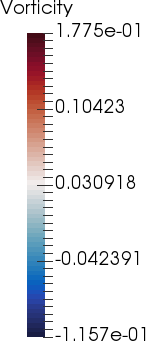
\includegraphics[width=\linewidth]{scale_vorticity.png}
\end{minipage}
\caption{\label{fig:top_4_events_vorticity} Vorticity field at $t=t^{\star}$ for the four highest drag fluctuations in the timeseries. The corresponding drag timeseries can be found in figure~\ref{fig:extremes_timeseries}.
  The high value for the drag results from the formation of a strong negative (red) vortex inducing a pressure drop at the base of the obstacle. The formation of such a structure is aided by important vorticity production at the bottom boundary of the obstacle coupled with the influence of positive vorticity in the vicinity of the base.}
\end{figure}  

% \begin{figure}
%   \centering
%   \begin{minipage}[h]{0.85\linewidth}
%     \begin{tabular}[h]{c|c}
%     \subfloat[$f'_d = 11.6\sigma$]{\label{fig:top_4_events_streamlines_a}\includegraphics[width=0.4\linewidth]{event_95_streamlines.png}} \hspace{0.5cm} & \hspace{0.5cm} \subfloat[$f'_d = 11.2\sigma$]{\includegraphics[width=0.4\linewidth]{event_69_streamlines.png}} \\
%     \hline
%     \subfloat[$f'_d = 10.6\sigma$]{\includegraphics[width=0.4\linewidth]{event_53_streamlines.png}} \hspace{0.5cm} & \hspace{0.5cm} \subfloat[$f'_d = 10\sigma$]{\includegraphics[width=0.4\linewidth]{event_20_streamlines.png}} 
%   \end{tabular}
% \end{minipage}
% \begin{minipage}[h]{0.1\linewidth}
%   \centering
%   \includegraphics[width=\linewidth]{scale_density.png}
% \end{minipage}
% \caption{\label{fig:top_4_events_streamlines} Density field at $t=t^{\star}$ for the four highest drag fluctuations in the control simulation for \tf{2}. Recall that the density $\rho$ is proportional to the pressure $p$, following the ideal gas state equation $p=c_s^2\rho$. See chapter~\ref{chap:test_flows} and appendix~\ref{app:lbm}. Additionally, velocity streamlines are depicted, representing advection by the flow at $t=t^{\star}$, see note~\ref{note:streamlines}. Blue areas indicate areas of lower pressure while red regions indicate regions of higher pressure. The formation of a vortex very close to the base boundary leads to a strong pressure drop. The downstream vortices originating from the top boundary layer separation are clearly visible and constrain the formation of the base vortex to a region very close to the base boundary.}
% \end{figure}

% \begin{figure}
%   \centering
%   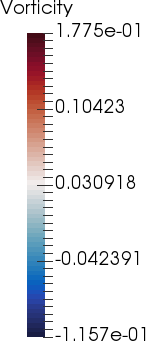
\includegraphics[width=0.1\linewidth]{scale_vorticity.png}
%   \begin{tabular}[h]{cccc}
%     \subfloat[$t = t^{\star}-0.54\tau_c$]{\label{frame_a}\includegraphics[width=.2\linewidth]{animation_event_95_0035}} & \subfloat[$t = t^{\star}-0.5\tau_c$]{\label{frame_b}\includegraphics[width=.2\linewidth]{animation_event_95_0036}} &     \subfloat[$t = t^{\star}-0.46\tau_c$]{\label{frame_c}\includegraphics[width=.2\linewidth]{animation_event_95_0037}} &     \subfloat[$t = t^{\star}-0.44\tau_c$]{\label{frame_d}\includegraphics[width=.2\linewidth]{animation_event_95_0038}} \\
%     \subfloat[$t = t^{\star}-0.4\tau_c$]{\label{frame_e}\includegraphics[width=.2\linewidth]{animation_event_95_0039}} &     \subfloat[$t = t^{\star}-0.36\tau_c$]{\label{frame_f}\includegraphics[width=.2\linewidth]{animation_event_95_0040}} &     \subfloat[$t = t^{\star}-0.34\tau_c$]{\label{frame_g}\includegraphics[width=.2\linewidth]{animation_event_95_0041}} &     \subfloat[$t = t^{\star}-0.3\tau_c$]{\label{frame_h}\includegraphics[width=.2\linewidth]{animation_event_95_0042}} \\
%     \subfloat[$t = t^{\star}-0.26\tau_c$]{\label{frame_i}\includegraphics[width=.2\linewidth]{animation_event_95_0043}} &     \subfloat[$t = t^{\star}-0.24\tau_c$]{\label{frame_j}\includegraphics[width=.2\linewidth]{animation_event_95_0044}} &     \subfloat[$t = t^{\star}-0.2\tau_c$]{\label{frame_k}\includegraphics[width=.2\linewidth]{animation_event_95_0045}} &     \subfloat[$t = t^{\star}-0.16\tau_c$]{\label{frame_l}\includegraphics[width=.2\linewidth]{animation_event_95_0046}} \\
%     \subfloat[$t = t^{\star}-0.12\tau_c$]{\label{frame_m}\includegraphics[width=.2\linewidth]{animation_event_95_0047}} &     \subfloat[$t = t^{\star}-0.08\tau_c$]{\label{frame_n}\includegraphics[width=.2\linewidth]{animation_event_95_0048}} &     \subfloat[$t = t^{\star}-0.04\tau_c$]{\label{frame_o}\includegraphics[width=.2\linewidth]{animation_event_95_0049}} &     \subfloat[$t = t^{\star}$]{\label{frame_p}\includegraphics[width=.2\linewidth]{animation_event_95_0050}} \\
%   \end{tabular}
%   \caption{\label{fig:type_1_event}Flow dynamics corresponding to a particular type 1 event, which drag timeseries and flow fields at $t=t^{\star}$ are displayed in figures~\ref{fig:extremes_timeseries}, \ref{fig:top_4_events_vorticity} and~\ref{fig:top_4_events_streamlines}, respectively. In each frame the vorticity field is displayed, as well as the velocity streamlines, representing advection by the flow at each instant. See note~\ref{note:streamlines} for a discussion of streamlines.
%     The maximum of the drag is attained for $t=t^{\star}$ and corresponds to frame~\ref{frame_p}.  The sequence starts with a shear boundary layer forming over the top boundary of the obstacle (frames~\ref{frame_a} to~\ref{frame_d}). This boundary layer separates (frames~\ref{frame_e} to~\ref{frame_j}) and results in the formation of a large positive eddy in the vicinity of the base of the obstacle (frames~\ref{frame_k} and~\ref{frame_l}). In the meantime, frames~\ref{frame_j} to~\ref{frame_m} depict the formation of an attached strong shear layer at the bottom boundary. Eventually, frames~\ref{frame_n} to~\ref{frame_p} illustrate that this results in vorticity production very close to the base, aided by the large positive eddy originating from the top boundary layer separation.}
% \end{figure}


We now describe the dynamics associated with some of the extreme drag fluctuations sampled in the contrl timeseries.
Figure~\ref{fig:top_four_events} displays the vorticity field at $t=t^{\star}$ for the four events with the larger fluctuation in the whole timeseries.
Remarkably, all four events display very similar flow configurations.
In each case, a strong vorticity region is located in the vicinity of the base of the obstacle, where vorticity levels can reach twice as much as the typical vorticity fluctuations displayed in figure~\ref{fig:typical_event}.
Such vorticity is produced through viscous shear along a boundary of the obstacle tangential to the mean flow direction.
By contrast with typical configurations, we observe that this vorticity is not directly advected by the mean flow, but instead constrained in the vicinity of the base of the obstacle.
Indeed, in each of the four examples displayed in figure~\ref{fig:top_four_events}, a large vortical region is located at roughly one obstacle length of the base.
As illustrated by the streamlines displayed in figure~\ref{fig:top_four_events_streamlines}, vorticity generated alongside the boundary has no other choice but to concentrate close to the base of the obstacle.

Figure~\ref{fig:dynamics} illustrates the dynamics leading to the extreme drag fluctuation corresponding to figure~\ref{fig:top_four_events_a}.
Figures~\ref{fig:dynamics_a} to~\ref{fig:dynamics_g} show that, from roughly $t^{\star}-\tau_c/2$ to $t^{\star}-\tau_c/3$, the top boundary layer is perturbed by an incoming eddy, advected by the flow above the obstacle.
The interaction of this eddy with the top boundary layer eventually leads to the formation of a region of negative vorticity at roughly one square length of the base of the obstacle.
This can be seen see in figure~\ref{fig:dynamics_k}.
Although this vorticity is too far from the base to directly affect the drag, it constrains the positive vorticity generated alongside the bottom boundary of the obstacle, as can be observed in figures~\ref{fig:dynamics_k} to~\ref{fig:dynamics_p}.

Figure~\ref{fig:top_four_events_timeseries} shows the drag timeseries corresponding to the four events featured in figure~\ref{fig:top_four_events}.
The timeseries are centered on the extreme event.
It illustrates that these fluctuations are short-lived, as their temporel extension is rouhly one correlation time unit.
This is the time it takes for the block eddy to form and be advected away by the mean flow, thus frreeing the vorticity concentrated in the vicinity of the base of the obstacle.

Among the $104$ sampled events, $80\%$ can be related to very similar dynamics as the one described in the previous paragraph. In order to identify such events, we monitored the averaged shear along the top or bottom booundary:
\begin{equation}
  \label{eq:avg_shear_def}
  \overline{\gamma} = \frac{1}{L} \int_{\mathcal{S}_b} \frac{\partial u_x(\mathbf{x})}{\partial y}\mathrm{d}\mathbf{x}
\end{equation}
where $L$ denotes the diameter of the cylinder, $u_x$ the longitudinal component of the velocity field and $\mathcal{S}_b$ the surface of either the top or the bottom boundary, depending on the event.
Figure~\ref{fig:type_1_and_type_2_a} displays the label of each sampled events, sorted according to the amplitude of the corresponding fluctuation.
It illustrates that the dynamics corresponding to the large majority of events also corresponds to the events with the hghest fluctuation amplitude.
Figure~\ref{fig:type_1_and_type_2_a} shows $\overline{\gamma}$ as a function of the instantaneous drag $f_d$, for $t^{\star}-2\tau_c \leq t \leq  t^{\star}+2\tau_c$, for each of these events.
For $t^{\star}-2\tau_c \leq t \leq t^{\star}-\tau_c$ and $t^{\star}+\tau_c \leq t \leq t^{\star}+2\tau_c$, paths concentrate in the region describing typical values for both $\overline{\gamma}$ and $f_d$.
As illustrated in figure~\ref{fig:extremes_timeseries}, the drag abruptly varies for $t^{\star}-\tau_c \leq t \leq t^{\star}+\tau_c$.
Correspondingly, paths in the $(f_d, \bar{\gamma})$ space display excursions to atypical values for both $\bar{\gamma}$ and $f_d$.
Interestingly, these excursions always go clockwise, that is, $\overline{\gamma}$ attains its maximum value before $f_d$ does.
This confirms that the increase of $\overline{\gamma}$ acts as a precursor for extreme drag fluctuations.

The remaining $20\%$ of the sampled events correspond to slightly different dynmaics.
In this case the vorticity responsible for the base pressure drop is not created along the top or bottom boundary, but directly through viscous shear alongside the base boundary of the obstacle.
This viscous shear is induced by a large vortex detached from the obstacle.

\subsection{Extreme fluctuations of the time-averaged drag }
\label{sec:time_avg}

% Motivation
In the previous section, we observed that rare events corresponding to extremely high values of the drag acting on the square obstacle have a lifetime of about $2\tau_c$.
In many applications, this duration is much smaller than the timescale of interest.
This is for instance the case when considering the interaction of a deformable structure with a turbulent flow: the typical response time may be much larger than the lifetime of drag fluctuations.

In such cases, a relevant observable is the \textit{time-averaged} drag
\begin{equation}
  \label{eq:def_time_averaged_drag}
  F_T(t) = \frac{1}{T}\int_t^{t+T} f_d(t) \mathrm{d}t,
\end{equation}
where $f_d$ denotes the instantaneous drag and $T\leq \tau_c$ a timescale of interest.
In the following we consider the case where $T \gg \tau_c$, typically $T=10\tau_c$.
In this context, a fluctuation of the average $F_T(t)$ is relatex to roughly $T / 2\tau_c$ independant fluctuations of $f_d$ over the time interval $[t;t+T]$.
What is the phenomenology leading to extreme values of $F_T(t)$ ?
Do an exceptionally large value of the average drag result from a single excpetionally large value of the instantaneous drag (case (1)) ?
Or from a succession of rather typical fluctuations, however all in the same direction (case (2)) ?
From the timeseries $\{f_d(t)\}_{0 \leq t \leq T_{tot}}$ we deduced the timeseries $\{F_T(t)\}_{0 \leq t \leq T_{tot}-T}$ and identified extreme positive fluctuations for which the drag exceeds a fixed threshold $a$ in the same way as described in section~\ref{sec:extreme_extraction}.
Setting $a=5.2\sigma _T$ leads to $84$ independant events, with $\sigma_T$ the standard deviation of the random process describing the time evolution of $F_T$.

Figure~\ref{fig:extreme_avg} displays the timeseries $\{f_d(t^{\star})\}_{t^{\star} \leq t \leq t^{\star}+T}$ for four of the highest fluctuations in the timeseries.
It illustrates that the phenomenology of the extreme fluctuations of the time-averaged drag cannot be reduced to the two above scenarios. 
Indeed, both case (1) and case (2) are featured in figure~\ref{fig:extreme_avg}, as well as intermediate cases where the very large value of the drag results from both a very large fluctuation and a large number of positive, rather typical, fluctuations.


This marginal phenomenology can be connected to the form of the tail of the \ac{pdf} describing extreme positive drag fluctations, illustrated in figure~\ref{fig:pdf_drag}. Let $X$ be a random variable whose \ac{pdf} is denoted $\mathbb{P}$ and standard deviation $\sigma_X$.
Considering an extreme positive value $a$ of $S_N=\sum_{n=1}{N}X_n$, the probability $p_1$(resp. $p_2$) of case (1) (resp. case (2)) writes:   
\begin{equation}
  \label{eq:indep}
  p_{1}(\sum_{1}^{N} X_n=a) \approx \mathcal{P}\left(\frac{a}{N}\right)^{N} \,\,\, \text{and} \,\,\, p_{2}(\sum_{1}^{N} X_n=a)\approx \mathcal{P}(a)  
\end{equation}
If $\mathbb{P}$ has an exponential posititve tail, \textit{i.e.} $\mathbb{P}(X=x) \underset{x \ll \sigma_X}{\propto} e^{-\alpha x}$, then both cases (1) and (2) are equiprobable, provided that the average $a=S_N/N$ is very large:
\begin{equation}
  \frac{p_{2}}{p_{1}} \underset{a\to \infty}{\sim} C\left(e^{-\alpha \frac{a}{N}}\right)^{N} e^{-\alpha a} = 1.
  \label{eq:ratio_exp}
\end{equation}

\section{Rare event algorithms}
\label{sec:rare_events_algorithms}

In the limit of very rare events, direct sampling approaches become unrealistic. As an example, consider the drag process $t \to f_d(t)$.
In the limit of extreme positive fluctuations, the return time of a fluctuations $f_d \geq a$ verifies
\begin{equation}
  \label{eq:return_time_scaling}
  r(a) \underset{a\to\infty}{\propto} \frac{1}{\mathbb{P}(f_d\geq a)} \propto e^{\alpha a}
\end{equation}
where $\alpha$ is the rate describing the positive tail of the drag \ac{pdf}, see figure~\ref{fig:pdf_drag}.
The computational cost required to sample events $f_d \geq a$ therefore scales like $e^{\alpha a}$.

In this section we discuss the application of rare event algorithms to the numerical sampling of extreme drag forces on immersed objects, on the example
of the flow presented in section~\ref{sec:test_flow}.
The purpose of these algorithm is to sample rare events for a computational cost well inferior to their return time.
Many of them rely on the simulation of an ensemble of trajectories in parallel, which can be duplicated or discarded from the ensemble depending on their relevance to
the realisation of extreme events of interest. 
Numerous algorithms and applications have been proposed since the original ideas of Kahn and Harris in the early 50s~\cite{kahnharris}, which can be sorted in two categories. On the one hand, \textit{splitting} approaches decompose rare events into a succession of less rare events that can be sampled with a higher probability.
On the other hand, \textit{importance sampling} relies on the sampling of trajectories according to a modified distribution, that is biased towards the rare events of interest.
In section~\ref{sec:ams}, we highlight that sampling  extreme flucutations of the instantaneous drag with the \ac{ams} algorithm is a difficult task.
In section~\ref{sec:gktl}, we apply an importance sampling algorithm, the \ac{gktl} algorithm, and efficiently sample rare trajectories corresponding to extreme flucutations of the time-averaged drag.
As an application, we use the \ac{gktl} algorithm to compute return times of very rare drag fluctuations.

\subsection{Extreme instantaneous drag forces with the \acl{ams} algorithm}
\label{sec:ams}

\subsection{Extreme time-averaged drag forces with the \acl{gktl} algorithm}
\label{sec:gktl}




\end{document}
%%% Local Variables:
%%% mode: latex
%%% TeX-master: t
%%% End:
